\section{Achieving conflict-freedom in POSIX}
\label{sec:sv6}

\XXX[STATUS]{Draft v2 ready.  Split from ``Finding scalability
  opportunities'' in SOSP.  Copied and reworked \refcache and \vm
  sections from EuroSys.  New intros for all subsections.

  Applied: Frans init-154-6dbae76, Eddie init-244-ga695479.

  Unapplied: Frans init-154-6dbae76 bigger change to \fs section,
  Eddie init-244-ga695479 restructuring comment in \vm section.
}

Given that many commutative operations are not conflict-free in Linux,
is it feasible to build file systems and virtual memory systems that
do achieve conflict-freedom for commutative operations?
%
To answer this
question, we designed and implemented a \code{ramfs}-like in-memory
file system called \fs and a virtual memory system called RadixVM for
\sys, our research kernel based on xv6~\cite{xv6}.
%
Although it is in principle possible to make the same changes in Linux,
we chose not to implement \fs in Linux because \fs's design
would have required extensive changes throughout the Linux kernel.
%
The designs of both RadixVM and \fs were guided by the
commutativity rule.  For \fs, we relied heavily on \tool throughout
development to guide its design and identify sharing problems in its
implementation.  \vm
was built prior to
\tool, but was guided by manual reasoning about commutativity and
conflicts (which was feasible because of the virtual memory system's
relatively simple interface).  We later validated \vm using \tool.

\begin{figure*}
\small
\centering
\inputnodraft{figures/testcases-sv6}
\caption{Conflict-freedom of commutative system call pairs in \sys.}
\label{fig:testcase-breakdown-sv6}
\end{figure*}

\Cref{fig:testcase-breakdown-sv6} shows the result of applying \tool
to \sys.  In contrast with Linux, \sys is conflict-free for nearly
every commutative test case.

For a small number of commutative operations, \sys is not
conflict-free.  Some appear to require implementations that would be
incompatible with conflict-freedom in other cases.  In these
situations, we preferred the conflict-freedom of the cases we
considered more important.  Other non-conflict-free cases represent
intentional engineering decisions in the interest of practical
constraints on memory consumption and sequential performance.  Complex
software systems inevitably involve conflicting requirements, and
scalability is no different.  However, the presence of the rule forced
us to explicitly recognize, evaluate, and justify where we made such
trade-offs.

The rest of \thiscref{sec:sv6} describes
the design of \sys and how it achieves conflict-freedom for cases
where current file and virtual memory systems do not.
%
\Thiscref{sec:sv6} starts with the design of Refcache, a scalable reference
counting mechanism used throughout \sys.  It then covers the designs
of RadixVM and \fs.  Finally, it discusses operations that are
difficult to make conflict-free without sacrificing other practical
concerns.

\subsection{Refcache: Scalable reference counting}
\label{sec:sv6:refcache}

Reference counting is critical to many OS functions and used
throughout \vm and \fs.  \vm must reference count physical pages
shared between address spaces, such as when forking a process, as well
as nodes in its internal radix tree.  Likewise, \fs must reference
count file descriptions, FD tables, and entries in various caches as
well as scalably maintain other counts such as link counts.
%
\Thiscref{sec:sv6:refcache} introduces \refcache, a novel reference
counting scheme
used by \vm and \fs.  \refcache implements space-efficient, lazy,
scalable reference counting using per-core \emph{reference delta
  caches}.  \refcache targets uses of reference counting that can
tolerate some latency in releasing reference counted resources and is
particularly suited to uses where increment and decrement operations
often occur on the same core (e.g., the same thread that allocated
pages also frees them).

% Since two virtual memory regions may share the same physical
% pages, such as when forking a process, \vm must have a way
% to decide when to free the underlying physical pages.  To do so,
% \vm reference counts each physical page, but a simple scheme with a
% single counter can result in scalability problems because threads will
% contend for the counter.  Likewise, \vm reference counts nodes of its
% radix tree to determine when they are empty; a single counter would
% cause operations on different parts of the node to contend.

Despite the seeming simplicity of reference counting, designing a
practical reference counting scheme that is conflict-free and scalable
for most operations turns out to be an excellent exercise in applying
the scalable commutativity rule to both implementation and interface
design.

In its simplest form, a reference counter has two operations,
\code{inc($o$)} and \code{dec($o$)}, which both return the new
reference count.  These operations trivially commute when applied to
different objects, so we focus on the case of a single object.  When
applied to the same object, these operations \emph{never} commute (any
reordering will change their responses) and cannot be made
conflict-free.

A better (and more common) interface returns nothing from \code{inc}
and, from \code{dec}, returns only an indication of whether the count
is zero.  This is equivalent to the Linux kernel's \code{atomic_inc}
and \code{atomic_dec_and_test} interface and is echoed in software
ranging from Glib to Python.  Here, a sequence of \code{inc} and
\code{dec} operations commutes if (and only if) the count does not
reach zero in any reordering.  In this case, the results of the
operations will be the same in all reorderings and, since reordering
does not change the final sum, no future operations can distinguish
different orders.  Therefore, by the scalable commutativity rule, any
such sequence has some conflict-free implementation.  Indeed,
supposing a \emph{particular} history with a commutative region, an
implementation can partition the count's value across cores such that
no per-core partition drops to zero in the commutative region.
However, a practical, \emph{general-purpose} conflict-free
implementation of this interface remains elusive.

\refcache exploits a further weakening of this interface, designed for
reference counters that can tolerate some latency between when the
count reaches zero and when the system detects that it's reached zero.
%
\XXX[AC]{Emphasize here that this is suitable for many uses of
  reference counting, like memory reclamation?}
%
In \refcache, \emph{both} \code{inc} and \code{dec} return nothing and
hence always commute, even if the count reaches zero.  A new
\code{review()} operation finds all objects whose reference counts
recently reached zero (and, in practice, calls their destructors).
\code{review} does not commute in any sequence where \emph{any}
object's reference count has reached zero and its implementation
conflicts on a small number of cache lines even when it does commute.
%
However, unlike \code{dec}, the system can control when and how often
it invokes \code{review}.
%
\sys invokes it
only at 10ms intervals---several orders of magnitude longer than the
time required by even the most expensive conflicts on current
multicores.
%
\refcache strikes a balance between broad conflict-freedom, strict
adherence to the scalable commutativity rule, and practical
implementation concerns, providing a general-purpose, efficient
implementation of an interface suitable for many uses of referencing
counting.

By separating count manipulation and zero detection, \refcache can
batch increments and decrements and
reduce cache line conflicts while offering an adjustable time bound
on when an object will be garbage collected after its reference count
drops to zero.  \code{inc} and \code{dec} are conflict-free with high
probability and \code{review} induces only a small constant rate of
conflicts for global epoch maintenance.

\refcache inherits ideas from sloppy
counters~\cite{boyd-wickizer:scaling}, Scalable NonZero Indicators
(SNZI)~\cite{snzi:podc}, distributed counters~\cite{appavoo:k42},
shared vs.\ local counts in Modula-2+~\cite{detreville:concurrent-gc},
and approximate counters~\cite{approx:counter}.
%
All of these techniques speed up increment and decrement operations
using per-core counters, but make different trade-offs between
conflict-freedom, zero-detection cost, and space.  With the exception
of SNZIs, these techniques do not detect when a count reaches zero, so
the system must poll each counter for this condition.  SNZIs detect
when a count reaches zero immediately, but at the cost of conflicts
when a count is small.  \refcache balances these extremes, enabling
conflict-free operations and efficient zero-detection, but with a
short delay.
%
Furthermore, in contrast with sloppy, SNZI, distributed, and
approximate counters, \refcache
requires space proportional to the sum of the number of reference
counted objects and the number of cores, rather than the product, and
the per-core overhead can be adjusted to trade off space and
scalability by controlling the reference delta cache collision rate.
%
Space overhead is particularly important for \vm, which must reference
count every physical page; at large core counts, other scalable
reference counters
would require more than half of physical memory just to track the
remaining physical memory.

\subsubsection{Basic \refcache}
In \refcache, each reference counted object has a global reference
count (much like a regular reference count) and each core also
maintains a local, fixed-size cache of deltas to objects' reference
counts.  Incrementing or decrementing an object's reference count
modifies only the local, cached delta and this delta is periodically
flushed to the object's global reference count.  The true reference
count of an object is thus the sum of its global count and any local
deltas for that object found in the per-core delta caches.  The value of the
true count is generally unknown, but we assume that once it drops to
zero, it will remain zero (in the absence of weak references, which
we discuss later).  \refcache depends on this stability to detect a
zero true count after some delay.

To detect a zero true reference count, \refcache divides time into
periodic \emph{epochs} during which each core flushes all of the
reference count deltas in its cache, applying these updates to the
global reference count of each object.  The last core in an epoch to
finish flushing its cache ends the epoch and all of the cores repeat
this process after some delay (our implementation uses 10ms).  Since
these flushes occur in no particular order and the caches batch
reference count changes, updates to the reference count can be
reordered.  As a result, a zero global reference count does not imply
a zero true reference count.  However, once the true count \emph{is}
zero, there will be no more updates, so if the global reference count
of an object drops to zero and \emph{remains} zero for an entire
epoch, then \refcache can guarantee that the true count is zero
and free the object.  To detect this, the first core that sets an object's
global reference count to zero adds the object to a per-core
\emph{review queue} and reexamines it two epochs later (which
guarantees one complete epoch has elapsed) to decide whether its true
reference count is zero.

\begin{figure*}
  \centering
  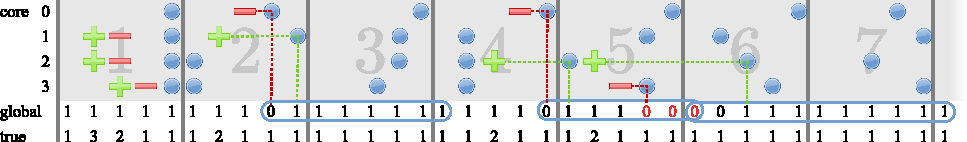
\includegraphics[width=\textwidth]{figures/refcache.pdf}
  \caption{\refcache example showing a single object over eight
    epochs.  Plus and minus symbols represent increment and decrement
    operations, dotted lines show when cores flush these to the object's
    global count, and blue circles show when each core flushes its
    local reference cache.  The loops around the global count show
    when the object is in core 0's review queue and
    the red zeroes indicate dirty zeroes.}
  \label{fig:refcache-ex}
\end{figure*}

\Cref{fig:refcache-ex} gives an example of a single object over
the course of eight epochs.  Epoch 1 demonstrates the power of
batching: despite six reference count manipulations spread over three
cores, the object's global reference count is never written to and
cache line conflicts arise only from epoch maintenance.  The
remaining epochs demonstrate the complications that arise from
batching and the resulting lag between the true reference count and
the global reference count of an object.

Because of the flush order, the two updates in epoch 2 are applied to
the global reference count in the opposite order of how they actually
occurred.  As a result, core 0 observes the global count temporarily
drop to zero when it flushes in epoch 2, even though the true count is
non-zero.  This is remedied as soon as core 1 flushes its increment,
and when core 0 reexamines the object at the beginning of epoch 4,
after all cores have again flushed their delta caches, it can see
that the global count is non-zero; hence, the zero count it observed
was not a true zero and the object should not be freed.

It is necessary but not sufficient for the global reference count to
be zero when an object is reexamined; there must also have been no
deltas flushed to the object's global count in the interim, even if
those changes canceled out or the deltas themselves were zero.
%
For example, core 0 will observe a zero global reference count
at the end of epoch 4, and again when it reexamines the object in
epoch 6.  However, the true count is not zero, and the global
reference count was temporarily non-zero during the epoch.  We call
this a \emph{dirty} zero and in this situation \refcache will
queue the object to be examined again two epochs later, in epoch 8.

\subsubsection{Weak references}
As described, \refcache is well suited to reference counts that track
the number of true references to an object, since there is no danger
of the count going back up from zero once the object becomes unreachable.
However, operating systems often need untracked references to objects;
for example, \fs's caches track objects that may be deleted at any time,
and may even need to bring an object's reference count back up from
zero.  \vm's radix tree has similar requirements.  To support such
uses, we extend \refcache with \emph{weak references}, which provide a
\code{tryget} operation that will either increment the object's
reference count (even if it has reached zero) and return the object,
or will indicate that the object has already been deleted.

A weak reference is simply a pointer marked with a ``dying'' bit,
along with a back-reference from the referenced object.  When an
object's global reference count initially reaches zero, \refcache sets
the weak reference's dying bit.  After this, \code{tryget} can
``revive'' the object by atomically clearing the dying bit and
fetching the pointer value, and then incrementing the object's
reference count as usual.  When \refcache decides to free an object,
it first atomically clears both the dying bit and the pointer in the
weak reference.  If this succeeds, it can safely delete the object.
If this fails, it reexamines the object again two epochs later.  In a
race between \code{tryget} and deletion, which operation succeeds is determined
by which clears the dying bit first.

This protocol can be extended to support multiple weak references per
object using a two phase approach in which all weak references are
first put in an intermediate state that can be rolled back if any
reference turns out to be revived.  Our current implementation does
not support this because it was not necessary for \vm or \fs.

\subsubsection{Algorithm}
\Cref{fig:refcache-code} gives pseudocode for \refcache.  Each core
maintains a hash table
storing its reference delta cache and the review queue that tracks
objects whose global reference counts reached zero.  A core reviews an
object after two epoch boundaries have passed, which guarantees
that all cores have flushed their
reference caches at least once.

\XXX![AC]{Make pseudo-code formatting consistent with rule chapter.}

\begin{figure}
  \def\fgap{-0.25em}            % Fit on a page
  \begin{tabbing}
    \quad\=\quad\=\quad\=\quad\=\quad\=\quad\=\kill
    inc(obj): \+\\
      if local cache[hash(obj)].obj $\ne$ obj: \+\\
        evict(local cache[hash(obj)]) \\
        local cache[hash(obj)] $\gets$ $\langle$obj, 0$\rangle$ \-\\
      local cache[hash(obj)].delta += 1 \\
    \-\\[\fgap]
    tryget(weakref): \+\\
      do: \+\\
        $\langle$obj, dying$\rangle$ $\gets$ weakref \-\\
      while weakref.cmpxchng($\langle$obj, dying$\rangle$,
        $\langle$obj, false$\rangle$) fails \\
      if obj is not null: \+\\
        inc(obj) \-\\
      return obj \\
    \-\\[\fgap]
    evict(obj, delta): \+\\
      % If this condition is true, then the locked region would be a
      % no-op, but why is it safe to do it without the lock?  The
      % danger is that the read of refcnt will slip in the middle of
      % another region that modified refcnt with obj locked.  evict
      % is the only place this happens and it does only a single write
      % to refcnt.  Assuming both this read and that write are
      % atomic, then we can consider this check atomic with the entire
      % locked region in the competing evict.
      if delta = 0 and obj.refcnt $\ne$ 0: return \\
      with obj locked: \+\\
        obj.refcnt $\gets$ obj.refcnt + delta \\
        if obj.refcnt = 0: \+\\
          if obj is not on any review queue: \+\\
            obj.dirty $\gets$ false \\
            obj.weakref.dying $\gets$ true \\
            add $\langle$obj, epoch$\rangle$ to the local review
            queue \-\\
          else: \+\\
            obj.dirty $\gets$ true \\
    \-\-\-\-\\[\fgap]
    flush(): \+\\
      evict all local cache entries and clear cache \\
      update the current epoch \\
    \-\\[\fgap]
    review(): \+\\
      flush() \\
      for each $\langle$obj, objepoch$\rangle$ in local review queue: \+\\
        if epoch $<$ objepoch + 2: continue \\
        with obj locked: \+\\
          remove obj from the review queue \\
          if obj.refcnt $\ne$ 0: \+\\
            obj.weakref.dying $\gets$ false \-\\
          else if obj.dirty or obj.weakref.cmpxchng(%
                $\langle$obj, true$\rangle$,
                $\langle$null, false$\rangle$) fails: \+\\
            obj.dirty $\gets$ false \\
            obj.weakref.dying $\gets$ true \\
            add $\langle$obj, epoch$\rangle$ to the local review queue \-\\
          else: \+\\
            free obj
  \end{tabbing}
  \vspace{-1em}                 % No idea where this space comes from
  \rule{\columnwidth}{0.5pt}
  \vspace{-\baselineskip}
  \caption[\refcache algorithm.]
  {\refcache algorithm.  Each core calls \code{review}
    periodically.  \code{evict} may be called by \code{flush} or because of a
    collision in the reference cache.  \code{dec} is identical to \code{inc} except
    that it decrements the locally cached delta.}
  \label{fig:refcache-code}
\end{figure}

All of the functions in \cref{fig:refcache-code} execute with
preemption disabled, meaning they are atomic with respect to each
other on a given core, which protects the consistency of per-core data
structures.  Fine-grained locks protect the \refcache-related fields
of individual objects.

For epoch management, our current implementation uses a barrier scheme
that tracks a global epoch counter, per-core epochs, and a count of
how many per-core epochs have reached the current global epoch.  This
scheme suffices for our benchmarks, but schemes with fewer cache-line
conflicts are
possible, such as the tree-based quiescent state detection used
by Linux's hierarchical RCU implementation~\cite{lwn:treercu}.

\subsubsection{Discussion}
\refcache trades latency for scalability by batching increment and
decrement operations in per-core caches.  As a result, except when
collisions in the reference delta cache cause evictions, \code{inc}
and \code{dec} are naturally conflict-free with all other operations.
%
Furthermore, because \refcache uses per-core caches
rather than per-core counts, it is more space-efficient than other
scalable reference counting techniques.  While not all uses of
reference counting can tolerate \refcache's latency, its scalability
and space-efficiency are well suited to the requirements of \vm and
\fs.

\XXX[Austin]{Design alternatives: token-passing or broadcast IPI for
epoch detection; lock-free versus fine-grained locking?}


\subsection{RadixVM: Scalable address space operations}

\XXX[AC]{``Disjoint'' instead of ``non-overlapping''?  Should at least
be consistent.}

The POSIX virtual memory interface is rife with commutativity, but
existing implementations scale poorly.  We model a virtual memory
system as four key logical operations: \code{mmap} adds a region of
memory to a process' virtual address space, \code{munmap} removes a
region of memory from the address space, and \code{memread} and
\code{memwrite} access virtual memory at a particular virtual address
or fail if no mapped region contains that address.  In reality, the
hardware implements \code{memread} and \code{memwrite} directly and
the VM system instead implements a \code{pagefault} operation; we
discuss this distinction below.

% Old, implementation-oriented text:
% A typical virtual memory system supports three key operations:
% \code{mmap} to add a region of memory to a process's virtual memory
% address space, \code{munmap} to remove a region of memory from the
% address space and the corresponding pages from the hardware page
% tables, and \code{pagefault}, which inserts a page into the hardware
% page tables at the faulting virtual address, allocating a new physical
% page if necessary.

% Old, more detailed memread/memwrite text:
% In reality, the hardware implements \code{memread} and \code{memwrite}
% directly using a cache of virtual-to-physical translations; when an
% operation misses in this translation cache, the hardware invokes
% \code{pagefault}, which is provided by the VM system.  This
% translation cache does not affect the interface specification or its
% commutativity; we'll discuss its effect on implementation below.

VM operations from \emph{different} processes (and hence address
spaces) trivially commute.  Most existing implementations use
per-process address space representations, so such operations are also
naturally conflict-free (and scale well).  VM operations from the same
process also often commute; in particular, operations on
\emph{non-overlapping} regions of the address space commute.
%
Many multithreaded applications exercise exactly this increasingly
important scenario: \code{mmap}, \code{munmap}, and related variants
lie at the core of high-performance memory allocators and garbage
collectors and partitioning the address space between threads is a key
design component of these
systems~\cite{ssmalloc:apsys,jemalloc,tcmalloc}.  Applications that
frequently map and unmap files also generate such workloads for the OS
kernel.

Unfortunately, owing to complex invariants in virtual memory systems,
widely used kernels such as Linux and FreeBSD protect each address
space with a single lock.  This induces not only conflicts but, often,
complete serialization between commutative VM operations on the same
address space, which can dramatically limit application
scalability~\cite{boyd-wickizer:scaling,clements:bonsai}.
\XXX{Mention workarounds or at least add that tidbit from Google?}

\vm is a novel virtual memory system in which commutative operations
on non-overlapping address space regions are almost always
conflict-free.  This ensures that if two threads operate on distinct
regions of virtual memory, the VM system does not limit the
application's scalability.  Furthermore, if multiple threads operate
on the same shared region, \vm constrains conflicts to the cores
executing those threads.

Achieving this within the constraints of virtual memory hardware,
without violating POSIX's strict requirements on the ordering and
global visibility of VM operations, and without unacceptable memory
overhead is challenging.  The following sections describe \vm's
approach.  \Cref{sec:radixvm:arch} describes the general architecture
of POSIX VM systems.  \Cref{sec:radixvm:tree,sec:radixvm:tlb} describe
the data structures that form the core of \vm.  Finally,
\cref{sec:radixvm:ops} describes how \vm uses these structures to
implement standard VM operations.


\XXX[AC]{Not sure where to say the following, but I think we need to
  be clear that none of these subsystems 100\% follows the rule, but
  that that's okay from an engineering standpoint:

  Like \refcache, \vm sacrifices strict adherence to the scalable
  commutativity rule in the interest of practical constraints on
  memory consumption and sequential performance.  Complex software
  systems inevitably involve conflicting requirements and scalability
  is no different.  However, in designing \vm, the presence of the
  rule forced us to explicitly recognize, evaluate, and justify where
  we made such trade-offs.}

\XXX![AC]{This uses subsubsections, but \refcache uses paragraphs.}

\XXX![AC]{Copy in some related work section bits from EuroSys.}

\subsubsection{POSIX VM architecture}
\label{sec:radixvm:arch}

\begin{figure}
  \centering
  \XXX!{Mapped regions, page tables, TLB with application on top.  See
    Bonsai Figure 1 and \vm talk.}
  \caption[Key structures in a POSIX VM system.]{Key structures in a
    POSIX VM system, showing an address space with four mapped
    regions.  Crossed-out page table entries are marked ``not
    present.''  Some pages have not been faulted yet, and thus are not
    present, despite being in a mapped region.}
  \label{fig:vm-structures}
\end{figure}

Between the POSIX VM interface on one side and the hardware virtual
memory interface on the other, \vm's general architecture necessarily
resembles typical Unix VM systems.  \Cref{fig:vm-structures} shows the
principle structures any Unix VM system must manage.  On the left is
the kernel's internal representation of the address space.  Logically,
this consists of a set of mapped regions of the virtual address space,
where each region may map either a file or ``anonymous'' (heap)
memory, has various access permissions, and may be either shared
across \code{fork} or copied.  \code{mmap} and \code{munmap} directly
manipulate this view of the address space.

However, translating virtual addresses to physical addresses is
ultimately performed in hardware---specifically by the memory
management unit (MMU)---and the MMU's representation of virtual memory
generally differs significantly from the kernel's internal
representation of the address space.  Most hardware architectures
specify some form of page table, like the x86 page table depicted in
\cref{fig:vm-structures}, for the kernel to inform the MMU of the
mapping from virtual addresses to physical addresses.  These
structures map addresses at a page granularity (typically 4~KB, though
most architectures also support larger pages) and represent access
permissions (which are checked by the MMU), but have little
flexibility.

While we model the VM system in terms of \code{mmap}, \code{munmap},
\code{memread}, and \code{memwrite}, only the first two are directly
implemented by the VM system.  The latter two are implemented by the
MMU using the kernel-provided page table.  However, the VM system has
a key hook into the MMU: when the virtual address of a read or a write
is marked ``not present'' in the page table or fails a permission
check, the MMU invokes the VM system's \code{pagefault} operation.
Modern Unix kernels exploit this mechanism to implement \emph{demand
  paging}, populating page table entries by allocating pages or
reading them from disk only once a page is first accessed, rather than
when it is mapped.
%
Hence, \code{mmap} and \code{munmap} simply clear the page table
entries of the region being mapped or unmapped; \code{mmap} depends on
\code{pagefault} operations to later fill these entries with mappings.
%
While demand paging significantly affects the implementation of the VM
system, it is nevertheless an implementation issue and does not affect
the commutativity of \code{memread} or \code{memwrite}.

The final key structure the VM system must manage is the hardware
translation lookaside buffer (TLB).  The TLB is a per-core associative
cache of virtual-to-physical mappings.  In architectures with a
hardware-filled TLB (x86, ARM, PowerPC, and many others), the MMU
transparently fills this cache from the page table.  Invalidating the
TLB, however, is the responsibility of the VM system.  Hence,
\code{munmap}, in addition to removing regions from the kernel's
internal address space representation and clearing entries in the page
table, must also invalidate the corresponding TLB entries.


\subsubsection{Radix tree}
\label{sec:radixvm:tree}

% At its core, an address space is a mapping from virtual addresses to
% physical addresses and metadata.  Hence, \vm needs a data structure
% that can track this mapping and support \code{mmap}ing and
% \code{munmap}ing ranges of virtual address space while avoiding
% conflicts between operations on disjoint regions.

We first tackle \vm's internal address space representation.
%
Widely-used operating system kernels represent an address space as a
balanced tree of mapped memory regions.  For example, Linux uses a
red-black tree~\cite{linux-source}, FreeBSD uses a splay
tree~\cite{freebsd-source}, and Solaris and Windows use AVL
trees~\cite{windows:wrk,windows:slides}).  This ensures fast lookups
and modifications for address spaces that can easily contain thousands
of mapped regions, but these data structures are poorly suited for
concurrent access: not only do they induce cache line conflicts
between operations on disjoint regions, they force all of these
kernels to use coarse-grained locking.

Lock-free data structures seem like a compelling solution to this
problem.  However, while lock-free data structures such as the Bonsai
tree used by the Bonsai VM~\cite{clements:bonsai} and lock-free skip
lists~\cite{herlihy:art} eliminate the coarse-grained serialization
that plagues popular VM systems, their operations are far from
conflict-free.  For example, \code{insert} and \code{lookup}
operations for a lock-free concurrent skip list can conflict on
interior nodes in the skip list---even when the \code{lookup} and
\code{insert} involve different keys and hence commute---because
\code{insert} must modify interior nodes to maintain $O(\log n)$
lookup time.  Indeed, any balanced data structure will suffer from
such problems.

A (completely impractical) way to achieve conflict-free commutative
operations is to represent a process's address space by storing the
metadata for each
virtual page individually in a large linear array indexed by virtual
page number.  In this linear representation, \code{mmap}, \code{munmap},
and \code{pagefault} can lock and manipulate precisely the pages being
mapped, unmapped, or faulted and operations on non-overlapping regions
are clearly conflict-free.  The design of \vm follows the same general
scheme as this strawman design, but reins in its memory consumption
using a multilevel, compressed radix tree.

\begin{figure}
\centering
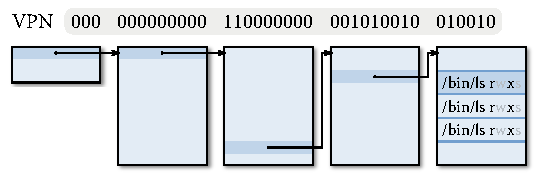
\includegraphics{figures/radix.pdf}
\caption{A radix tree containing both an anonymous mapping
  and a file mapping.  Blue indicates the path for looking up the 36-bit
  virtual page number shown in bits at the top of the figure.  The last
  level of the tree contains separate mapping metadata for each page.
}
\label{fig:radix}
\end{figure}

The index data structure of \vm resembles a hardware page table
structurally, storing mapping metadata in a fixed-depth radix tree,
where each level of the tree is indexed by nine (or fewer) bits of the
virtual page number (\cref{fig:radix}).  Like the linear array,
the radix tree supports only point queries (not range queries) and
iteration, but unlike the linear array, \vm can compress repeated
entries and lazily allocate the nodes of the radix tree.  Logically,
any node that would consist entirely of identical values is folded
into a single value stored in the parent node.  This continues up to
the root node of the tree, allowing the radix tree to represent vast
swaths of unused virtual address space with a handful of empty slots
and to set large ranges to identical values very quickly.  This
folding comes at a small cost: operations that expand a subtree will
conflict with other operations in that same subtree, even if their
regions do not ultimately overlap.  However, after initial address
space construction, the radix tree is largely ``fleshed out'' and
these initialization conflicts becomd rare.

To record each mapping, \vm stores a separate copy of the mapping metadata
in the radix tree for each page in the mapped range.  This differs
from a typical design that allocates a single metadata object
to represent the entire range of a mapping (e.g., ``virtual memory
areas'' in Linux).
%
This is practical because \vm's mapping metadata object is small and
designed so that it will initially be byte-wise
identical for every page of a mapping, meaning that large mappings can
created efficiently and folded into just a few slots in the radix
tree's nodes.

Also unlike typical virtual memory system designs, \vm stores pointers
to physical memory pages in the mapping metadata for pages that have
been allocated.  This is easy to do in \vm because, modulo folding,
there is a single mapping metadata object for each page.  It's also
important to have this canonical representation of the physical memory
backing a virtual address space because of the way \vm handles TLB
shootdown (see \cref{sec:radixvm:tlb}).  This does increase the space
required by the radix tree, but, asymptotically, it's no worse than
the hardware page tables, and it means that the hardware page tables
themselves are cacheable memory that can be discarded by the OS to
free memory.

To keep the memory footprint of the radix tree in check, the OS must be
able to free nodes that no longer contain any valid mapping metadata.
To accomplish this without introducing undue conflicts, we leverage
\refcache to scalably track the number of used slots in each node.
When this count drops to zero, the radix tree can remove the node from
the tree and delete it.  Since \vm may begin using a node again before
\refcache reconciles the used slot count, nodes link to their children
using weak references, which allows the radix tree to revive nodes
that go from empty to used before \refcache deletes them, and to
safely detect when an empty child node has been deleted.

Collapsing the radix tree does potentially introduce conflicts;
however, unlike with eager garbage collection schemes, rapidly
changing
mappings cannot cause the radix tree to rapidly delete and recreate
nodes.  Since a node must go unused for at least two \refcache epochs
before it is deleted, any cost of deleting or recreating it (and any
additional contention that results) is amortized.
\XXX[AC]{We don't actually implement this, but if we did, when we
analyze performance without \refcache, things would be even worse.
Might be worth mentioning.}

In contrast with more traditional balanced trees, using a radix tree
to manage address space metadata allows \vm to achieve near-perfect
conflict-freedom (and hence scalability) for metadata operations on
non-overlapping regions of an address
space.  This comes at the cost of a potentially larger memory
overhead; however, address space layouts tend to exhibit good
locality and folding efficiently compresses large ranges, making radix
trees a good fit for a VM system.
\XXX[AC]{We show this in the \vm paper.  Pull that in here or in the
  evaluation?}

\subsubsection{TLB management}
\label{sec:radixvm:tlb}

The other major impediment to scaling \code{mmap} and \code{munmap}
operations is the need to explicitly invalidate cached
virtual-to-physical mappings in per-core TLBs when a page is unmapped
(or remapped).
%
Because TLB shootdowns must be performed on every CPU that may have
cached a page mapping that's being modified, and because hardware does
not provide
information about which CPUs may have cached a particular mapping,
typical Unix VM systems send TLB shootdown interrupts to all
CPUs using the modified address space, inducing cache line conflicts
and limiting scalability.

\vm addresses this problem by precisely tracking the set of CPUs that
have accessed each page mapping.
%
In architectures with software-filled TLBs (such as the MIPS or
UltraSPARC) this is easy, since the MMU informs the kernel of each
miss in the TLB.  The kernel can use these TLB miss faults to track
exactly which CPUs have a given mapping cached and, when a later
\code{mmap} or \code{munmap} changes this mapping, it can deliver
shootdown requests
only to cores that have accessed this mapping.  On architectures
with hardware-filled TLBs such as the x86, \vm achieves the
same effect using per-core page tables.
%
With TLB tracking, if an application thread
allocates, accesses, and frees memory on one core, with no other threads
accessing the same memory region, then \vm will perform no TLB shootdowns.

The obvious downside to this approach is the extra memory required for
per-core page tables.  We show in \cref{eval:memory} that this
overhead is small in practice compared to the total memory footprint
of an application, but for applications with poor partitioning, it may
be necessary for the application to provide hints about widely shared
regions so the kernel can share page tables (similar to Corey address
ranges~\cite{boyd-wickizer:corey}) or for the kernel to detect such
regions.
%
\XXX![AC]{Do we show this in \cref{eval:memory}?}
%
The kernel could also reduce overhead by simply discarding page table
pages when memory is low.

\subsubsection{VM operations}
\label{sec:radixvm:ops}

With the components described above, \vm's implementation of the core
VM operations is surprisingly straightforward.
%
One of the most difficult aspects of the POSIX VM interface in a
multicore setting is its strict ordering and global visibility
requirements~\cite{clements:bonsai}.  For example, after the return
of an \code{munmap}, no thread on any core should be able to access
the unmapped
region.  Similarly, after \code{mmap} returns, any thread on any core
must be able to access the mapped region.  Furthermore, though not
required by POSIX, it is generally assumed that these operations are
atomic.

\vm enforces these semantics by always locking, from left to right,
the bottom-most radix tree entries for the region of an operation.
This simple mechanism ensures all operations on an address space are
linearizable~\cite{herlihy:linearizability} and, for fully expanded
subtrees, prevents cache line conflicts between operations on disjoint
regions.

% When locking a region that has not been expanded out to leaf nodes
% yet, \vm acquires locks on the corresponding internal node slots
% instead.  When \vm expands the tree by allocating new nodes, it
% propagates the lock bit to every entry in the newly allocated node,
% and unlocks the parent interior node slot.  Releasing the lock
% clears the lock bits in the newly allocated child node.  Tree
% traversal does not require locks or indeuce conflicts because it
% increments each node's reference count through a \refcache weak
% reference.

An \code{mmap} invocation, like all \vm operations, first locks the
range being mapped.
%
If there are existing mappings within the
range, \code{mmap} unmaps them, as described later for \code{munmap}.
\code{mmap} then fills in mapping metadata for the new mapping (protection
level and flags arguments to \code{mmap}, as well as what backs this virtual
memory range, such as a file or anonymous memory).  If the mapping covers
an entire radix tree node, and the child nodes have not been allocated
yet, the radix tree collapses the mapping metadata into a single slot
in the interior of the tree.
Otherwise, \vm copies the mapping metadata into each leaf node entry in
the range.  Finally, \vm unlocks the range.  Like in other VM systems,
\code{mmap}
doesn't allocate any physical pages, but leaves that to \code{pagefault},
so that pages are allocated only when they are used.

A \code{pagefault} invocation traverses the radix tree to find the
mapping metadata for the faulting address, and acquires a lock on it.
It then allocates a physical page if one has not been allocated yet
(for anonymous memory), or fetches it from the buffer cache (for file
mappings) and
stores it in the mapping metadata.  Finally, \code{pagefault} fills in the
page table entry in the local core's page table, and adds the local core
number to the TLB shootdown list in the mapping metadata for that address.
\code{pagefault} then releases the lock and returns.

To implement \code{munmap}, \vm must clear mapping metadata from the
radix tree, clear page tables, invalidate TLBs, and free physical
pages.  \code{munmap} begins by locking the range being unmapped,
after which it can scan the region's metadata to gather references to
the physical pages backing the region, collect the set of cores that
have faulted pages in the region into their per-core page tables, and
clear each page's metadata.  It can then send inter-processor
interrupts to the set of cores it collected in the first step.  These
interrupts cause the remote cores (and the core running \code{munmap})
to clear the appropriate range in their per-core page table and
invalidate the corresponding local TLB entries.  Once all cores have
completed this shootdown process, \code{munmap} can safely release its
lock on the range and decrement the reference counts on the physical
pages that were unmapped.

Note that an invocation of \code{pagefault} on one core may concurrently
access a page that another core is in the process of unmapping,
but the mapping metadata lock makes this work out correctly: either
\code{pagefault} acquires the lock first or \code{munmap} does.  In the
first case, the page fault succeeds, which is okay since the pages must be
inaccessible only after \code{munmap} returns.  In the second case,
\code{munmap} runs first and removes the mapping for the unmapped range
before releasing the locks. Then, \code{pagefault} will see that there
is no mapping for the faulting address and will halt the faulting thread.

\subsubsection{Discussion}

By combining \refcache for scalable reference counting, radix trees
for maintaining address space metadata, and per-core page tables for
precise TLB tracking and shootdown, \vm achieves conflict-freedom for
the vast majority of commutative VM operations.  The clear
commutativity properties of the POSIX VM interface, combined with the
right data structures makes this possible with a straightforward
concurrency plan based on precise range locking.
%
As shown in \cref{fig:testcase-breakdown-sv6}, \tool confirmed that
most commutative operations in \vm are conflict-free.  In
\cref{sec:eval}, we further confirm that \vm's design translates into
scalable performance for application workloads. \XXX![AC]{Do we
  confirm this?}


\subsection{\fs: Conflict-free file system operations}

\XXX[FK/AC]{Make this more like \vm section.  Lead with operations and
  their rough commutativity.  Since the high-level structure is much
  more like a conventional VFS than \vm is like a conventional VM, say
  that and then explain some key detail (probably something involving
  hash tables).  E.g., how the inode cache works.  (See FK edits for
  init-154-6dbae76)}

\fs encompasses \sys's unified buffer cache and VFS layers, providing
operations such as \code{read}, \code{write}, \code{open}, and
\code{unlink}.  We focused on the VFS and buffer cache layers because
these are the common denominators of all file systems in a Unix
kernel.
%
In contrast with \vm,
\fs makes extensive use of well-known techniques for scalable
implementations, such as per-core resource
allocation, double-checked locking, lock-free readers using
RCU~\cite{rcu:linux},
and seqlocks~\cite[\S6]{lameter:linuxsync}.
%
\fs also employs \refcache for tracking both internal resources and
inode link counts.
%
\fs is also structured much like contemporary Unix VFS subsystems,
with inode and directory caches represented as concurrent hash tables
and per-file page caches.
%
What sets \fs apart is that the details of its implementation were
guided by the scalable commutativity rule and, in particular, by
\tool.
%
This led to several common design patterns, which we illustrate with
example test cases from \tool{}:
%
\XXX[AC]{\fs is more irregular than \vm, so \tool was more important.}


\paragraph{Layer scalability.}  \fs uses data structures that
themselves naturally satisfy the commutativity rule, such as linear
arrays, radix trees, and hash tables.  In
contrast with structures like balanced trees, these data
structures
typically share no cache lines when different elements are accessed
or modified.  For example, \fs stores the cached data pages for a given inode
using a radix tree, so that concurrent reads or writes to different
file pages scale, even in the presence of operations
extending or truncating the file.
% , as long as they don't access the part
% of the file that's being extended or truncated.
\tool led us to an additional benefit of this representation:
many operations also use this radix tree to determine if some offset
is within the file's bounds without reading the size and conflicting
with operations
that change the file's size.
%
For example, \code{pread} first probes this radix tree for the
requested read offset: if the offset is beyond the last page of the
file, it can return 0 immediately without reading (and potentially
conflicting on) the file size.

\XXX[FK]{``Defer work'' can be presented as dealing with
  non-commutative ops.}

\paragraph{Defer work.} Many \fs resources are shared,
such as file descriptions and inode objects, and must be freed when no
longer referenced.
Typically, kernels release resources immediately, but this requires
eagerly tracking references to resources, causing
commutative operations that access the same resource to conflict.  Where
releasing a resource is not time-sensitive, \fs
uses Refcache to batch reference count
reconciliation and zero detection.  This way, resources are eventually
released, but within each Refcache epoch commutative operations can be
conflict-free.

\XXX[AC]{Discuss crazy pipe hybrid reference counting scheme?}

Some resources are artificially scarce, such as inode numbers in a typical
Unix file system.  When a typical Unix file system runs out of free
inodes, it must reuse an inode from a recently deleted file.
%
This requires finding and garbage collecting unused inodes, which
induces conflicts.
%
However,
the POSIX interface does not require that inode numbers be reused, only
that the same inode number is not used for two files at once.  Thus,
\fs never reuses inode numbers.  Instead, inode numbers are
generated by a monotonically increasing per-core counter, concatenated
with the core number that allocated the inode.  This allows \fs to defer
inode garbage collection for longer periods of time, and enables
conflict-free and scalable
per-core inode allocation.


% \paragraph{Check before updating.}  Before updating any data structure,
% \fs first checks whether the data structure already contains the new
% value, and avoid any writes if so.  For example, the Linux file system
% always acquires a lock on an inode when truncating the file.  This means
% that concurrent truncate operations do not scale, even if the file
% is already empty.  \fs first checks the current length of the file,
% and avoids updating the length or acquiring any locks if the file is
% already at the right size.

% As another example, if one thread tries to create an existing file using
% \code{open(O_CREAT|O_EXCL)}, it should fail, but a na\"ive implementation
% might first acquire a lock to prepare for creating the file, and then
% check whether the file already exists.  This makes
% concurrent \code{open(O_CREAT|O_EXCL)} calls for an existing file name
% non-scalable.  \fs first checks whether the file already exists without
% modifying any cache lines, making these operations scale.

% \XXX[AC]{The above two examples are slightly off.  E.g., if I do two
% truncates and the first writes to the file length and the second reads
% that, that's sharing.  These are both idempotent updates, which is one
% of the few things we \emph{don't} do scalably.}

% As a final example, if two file names \code{a} and \code{b} point to the
% same inode, \code{rename(a, b)} should remove the directory entry for
% \code{a}, but it should not modify the directory entry for \code{b}, since
% it already points at the right inode.  By checking the directory
% entry for \code{b} before updating it, \fs allows \code{rename(a, b)}
% to scale with other operations that look up \code{b}.


\paragraph{Precede pessimism with optimism.} Many operations
in \fs have an optimistic check stage followed by a pessimistic update
stage, a generalized sort of double-checked locking.  The optimistic
stage checks conditions for the operation and returns immediately if
no updates are necessary (this is often the case for error returns,
but can also happen for success returns).  This stage does no writes
or locking, but because no updates are necessary, it is often easy to
make atomic.  If updates are necessary, the operation acquires
locks or uses lock-free protocols, re-verifies its conditions to
ensure atomicity of the update stage, and performs updates.  For
example, \code{lseek} first computes the new offset using a lock-free
read-only protocol and returns early if the new offset is invalid or
equal to the current offset.  Otherwise, \code{lseek} locks the file
offset and re-computes the new offset to ensure consistency.
%
In fact, \code{lseek} has surprisingly complex interactions with
system state and other operations, and arriving at a protocol that was
both correct and conflict-free in all commutative cases would have
been difficult without \tool.

\code{rename} is similar.  If two file names \code{a} and \code{b}
point to the
same inode, \code{rename(a, b)} should remove the directory entry for
\code{a}, but it does not need to modify the directory entry for
\code{b}, since
it already points at the right inode.  By checking the directory
entry for \code{b} before updating it, \code{rename(a, b)} avoids
conflicts with other operations that look up \code{b}.
%
As we saw in \cref{sec:topic:rename-conditions}, \code{rename} has
many surprising and subtle commutative cases and, much like
\code{lseek}, \tool was instrumental in helping us arrive at an
implementation that was conflict-free in these cases.


\paragraph{Don't read unless necessary.}  A common internal interface
in a file system implementation is a \code{namei} function that
checks whether a path name exists, and if so, returns the inode for
that path.
%
However, reading the inode is unnecessary
if the caller wants to know only whether a path name existed, such as
an \code{access(F_OK)} system call.  In particular, the \code{namei}
interface makes it impossible for concurrent \code{access(b, F_OK)}
and \code{rename(a, b)} operations to scale when \code{a} and \code{b}
point to different inodes, even though they commute.
\fs has a separate internal interface to check for existence of a
file name, without looking up the inode, which allows \code{access}
and \code{rename} to scale in such situations.


\subsection{Difficult-to-scale cases}

As \cref{fig:testcase-breakdown-sv6} illustrates, there are a few
(\pyexpr{mscan.xv6.shared} out of \pyexpr{mscan.ntestcases})
commutative test cases for
which \vm and \fs are not conflict-free.
%
The majority of these tests involve idempotent updates to internal
state, such as two \code{lseek} operations that both seek a file
descriptor to the same offset, or two anonymous \code{mmap} operations
with the same fixed base address and permissions.  While it is
possible implement these scalably, every implementation we considered
significantly impacted the performance of more common operations, so
we explicitly chose to favor common-case performance over total
scalability.  Even though we decided to forego scalability in these
cases, the commutativity rule and \tool forced us to consciously make
this trade-off.
%
\XXX[AC]{About 75\% are known idempotent.}

% Non-idempotent shared case list (incomplete):
% close_close_pe_5: Closing pipe writer (eager counting)
% close_read_pdc_0: Closing pipe writer, reading writer always EBADF
% close_write_pd8_0: Symmetric to close_read_pdc_0
% lseek_read_pad8_2: Reading nothing from two different offsets
% lseek_read_p8b6_3: Same as lseek_read_pad8_2
% mmap_mprotect_pf8_41: Making different read-only mappings read-only
%   (The mprotect is a no-op, but what it reads is modified)
% mmap_mprotect_pae_40: Same
% read_read_pce4_0: Two reads from a file full of zeroes
% read_write_pbb0_2: Reading nothing from different end-of-file offsets
% write_write_pff8_1: Writing to a pipe with no readers
%   (We could probably fix this one)
% write_write_pff8_2: Same
% write_write_pf78_1: Same

Other difficult-to-scale cases are more varied.  Several involve
reference counting of pipe file descriptors.  Closing the last file
descriptor for one end of a pipe must immediately affect the other
end; however, since there's generally no way to know a priori if a
\code{close} will close the pipe, a shared reference count is used in
some situations.  Other cases involve operations that return the same
result in either order, but for different reasons, such as two reads
from a file filled with identical bytes.
%
By the rule, each of these cases has some conflict-free
implementation, but making these particular cases conflict-free would
have required sacrificing the conflict-freedom of many other
operations.


\XXX[AC]{fstest works around all radix tree expansion.  Is this
cheating?  That's actually an interesting case.}

\XXX[AC]{Summarize or something?}
